\section{Introductie}


\subsection{Aanleiding en Context}

Voortman Machinery, gevestigd in Rijssen is producent van geavanceerde metaalbewerkingsmachines. Voortman is opgericht in 1968 \cite{web:VoortmanGeschiedenis}. In het begin richtte Voortman zich vooral op de productie van staalconstructies. In 1995 begon Voortman ook staalbewerkingsmachines te ontwikkelen en te produceren waaruit de naam Voortman Steel Machinery is ontstaan. In de loop der jaren is het bedrijf uitgegroeid tot een wereldwijde fabrikant van \gls{cnc}-staalbewerkingsmachines met hierbij ook de bijpassende softwareoplossingen.

\vspace{1cm}

 In veel machines van Voortman zitten spindels, deze spindels worden gebruikt in de machines om bijvoorbeeld te vrezen, tapen of boren. Na een bepaalde tijd kunnen deze spindels door slijtage of schade niet meer correct functioneren. Deze spindels kunnen in veel gevallen nog gereviseerd worden, dit kan echter veel geld kosten wanneer deze worden opgestuurd naar de fabrikant.
 
 \vspace{1cm}
 
  Voortman wil daarom de spindels zelf kunnen reviseren. Echter ondersteunt de huidige testkast (figuur \ref{fig:TestKastFoto}) bij Voortman slechts één soort spindel terwijl er wel veel verschillende soorten gebruikt worden in het machine portfolio van Voortman. Hieruit kwam de opdracht om de testkast aan te passen zodat zo veel mogelijk soorten spindels kunnen worden getest op de testkast van Voortman zelf.

\begin{figure}[h]
	\centering
	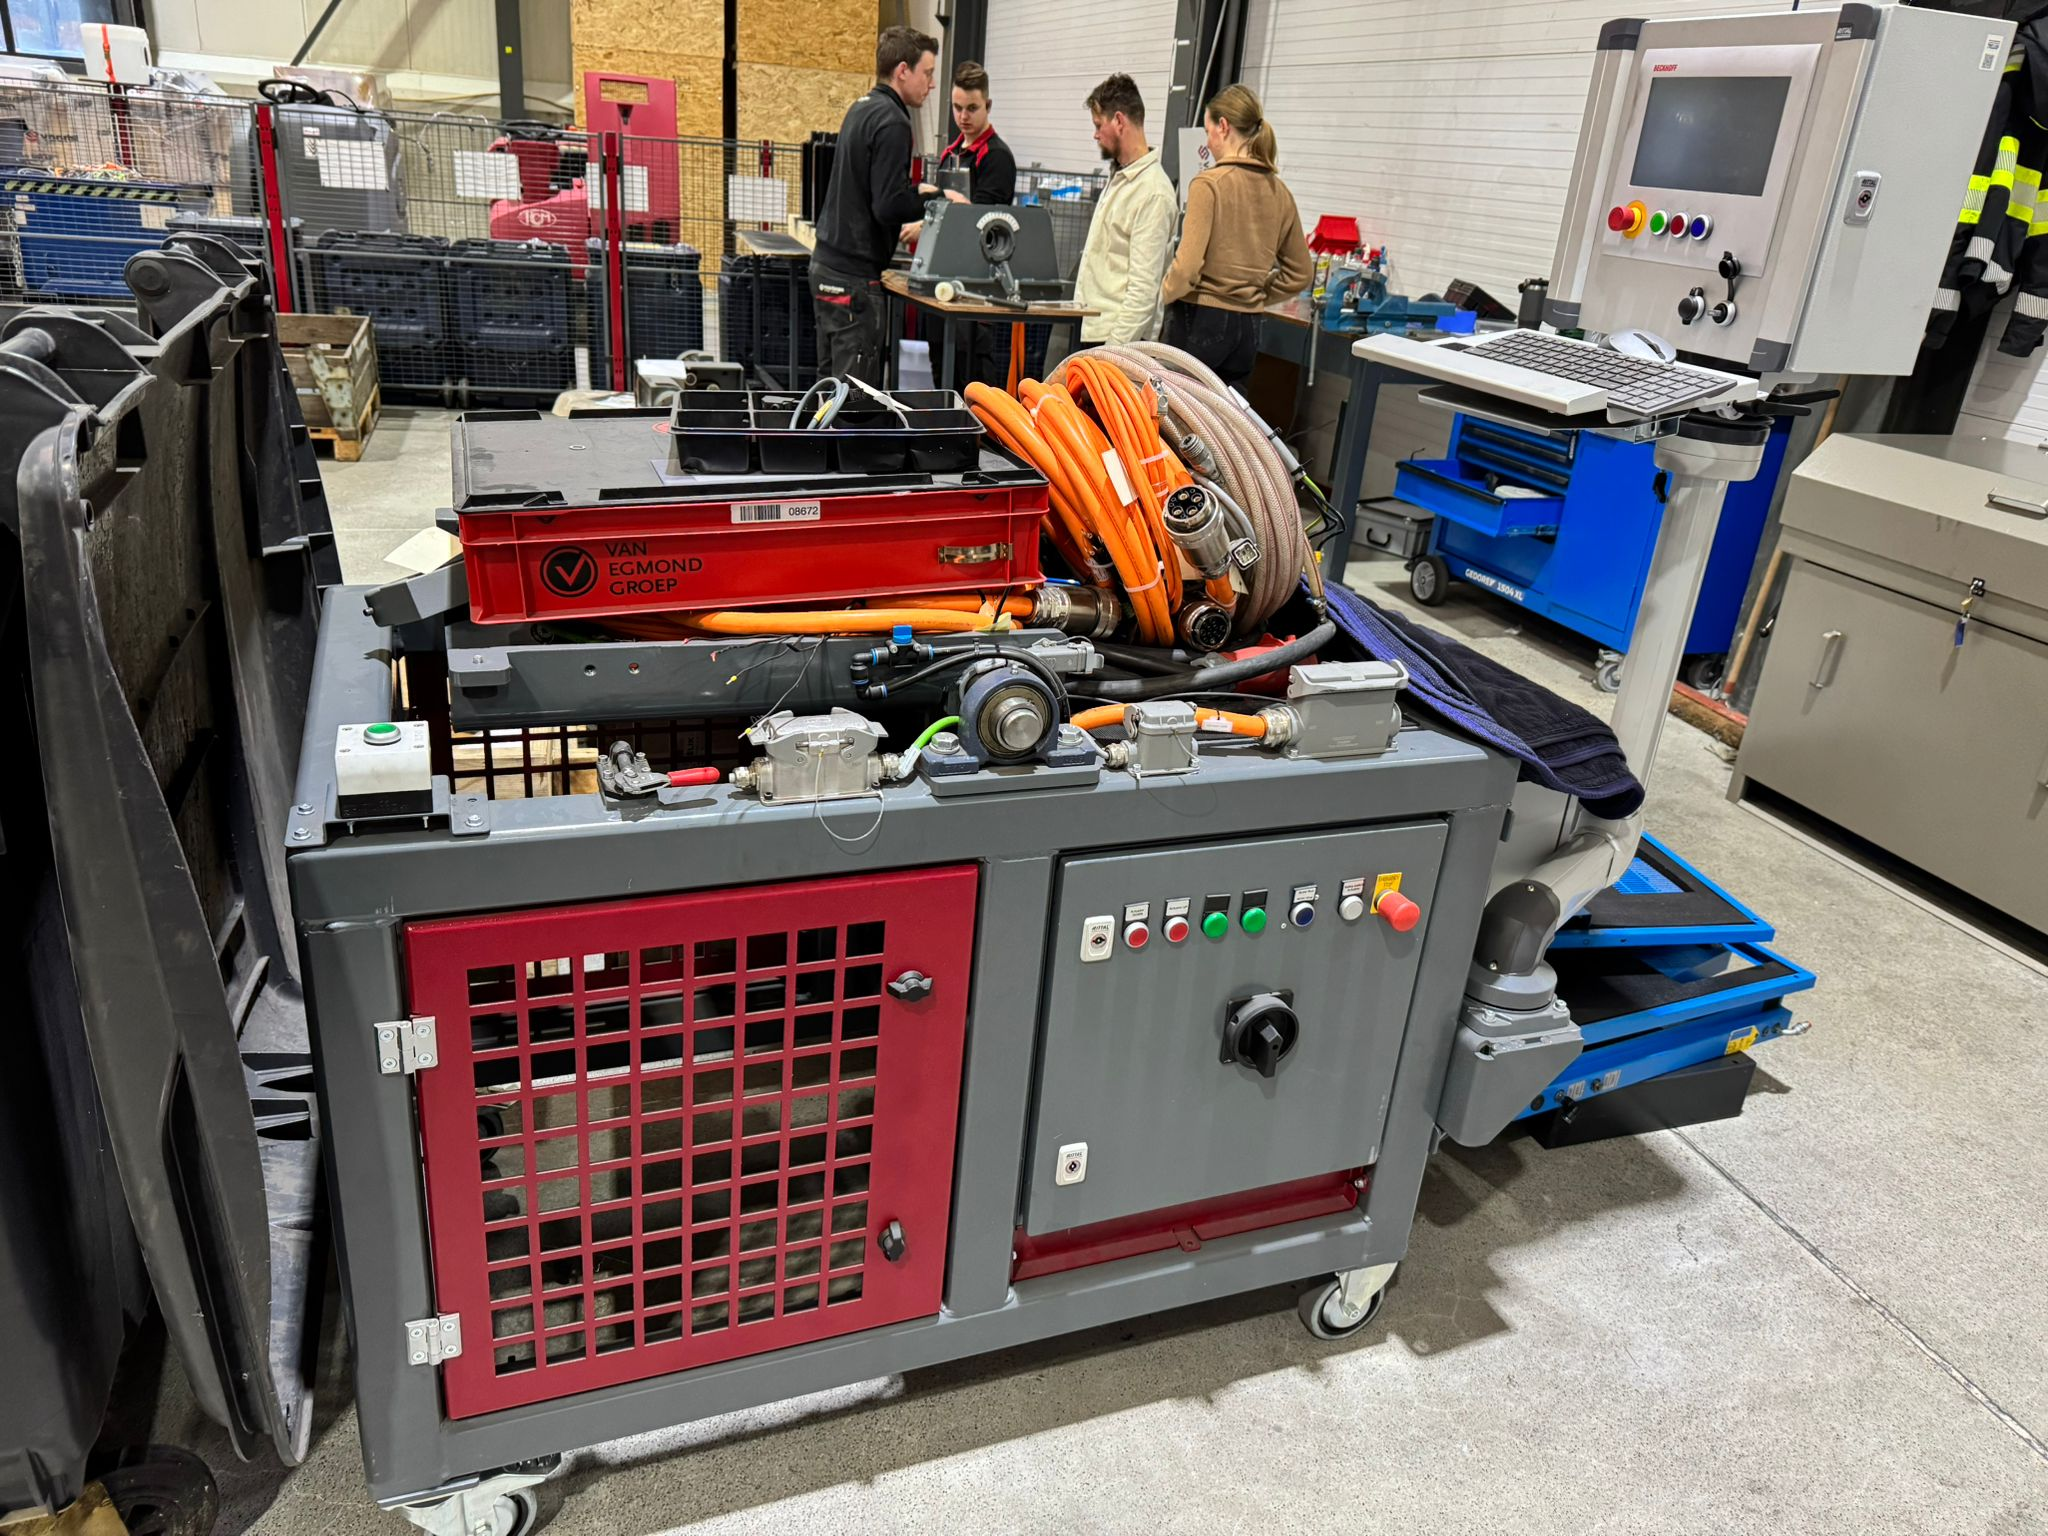
\includegraphics[width=300pt]{TestKast}
	\label{fig:TestKastFoto}
	\caption{Foto van de bestaande testkast}
\end{figure}

\newpage

\subsection{Doelstelling}



\subsection{Onderzoeksvragen}

Tijdens de afstudeerperiode zullen de volgende onderzoeksvragen beantwoord worden:

\begin{enumerate}
	\item Welke motorparameters in de drive zijn relevant om verschillende motortypes aan te sturen?
	
	\item Hoe kunnen motorparameters eenvoudig en automatisch in de drive geschreven worden?
	
	\item Welke encoderinterfaces moeten er allemaal ondersteunt worden zodat alle motortypes die Voortman wil testen aangesloten kunnen worden?
	
	\item Hoe kan een elektromotor effectief worden getest en welke parameters in de drive kunnen worden gebruikt om de prestaties te analyseren?
	
	\item Hoe kan de software automatisch rapporten genereren die de prestaties van de motoren beschrijven, inclusief waarschuwingen bij afwijkingen (bijv. te hoge trillingen, overbelasting)?
	
	\item Hoe kan de testkast worden aangepast om nieuwe motortypes (met andere parameters en communicatieprotocollen) in de toekomst gemakkelijk te integreren?
\end{enumerate}

\subsection{Afbakening}

